\chapter{Next steps}
\label{ch:next-steps}

With the dataset assembled, cleaned and characterised (Chapter~\ref{ch:dataset}),
the analysis proceeds as follows.

\section{Observables on the whole trajectory}
\label{sec:obs-global}
A first group of observables requires \emph{no} segmentation: it can be measured directly on
the full trajectories and already probes the transport at the global level.

\begin{description}
  \item[Mean-squared displacement (MSD).] With every flight starting at the origin
        ($\mathbf{r}(0)=\mathbf{0}$), the \emph{ensemble-averaged} MSD is the mean squared
        horizontal distance reached after an elapsed time $t$,
        \begin{equation}
          \mathrm{MSD}(t)=\big\langle\,|\mathbf{r}(t)|^2\big\rangle,
        \end{equation}
        where $\langle\cdot\rangle$ is an average \emph{over flights} (an ensemble average) at
        fixed $t$. Its growth law
        $\mathrm{MSD}(t)\sim t^{\alpha}$ fixes the transport regime ($\alpha=1$ Brownian,
        $\alpha>1$ super-diffusive, $\alpha<1$ sub-diffusive; equivalently the Hurst exponent
        $H=\alpha/2$). This is the primary test for anomalous transport. \rev{On this
        archive it is measured together with the time average below and read against it:
        the ensemble curve is synchronised at take-off and turns out to cross over where
        the population leaves its launch area, so what it yields is that timescale rather
        than a single $\alpha$, and the exponent is read off the time average.}
  \item[Time-averaged MSD (TA-MSD).] A second MSD estimator is built entirely
        \emph{within} a single flight. For flight $k$ of duration $T_k$, one slides a window
        of width $t$ along the trajectory $\mathbf{r}^{(k)}$ and averages the squared
        displacement over all starting times $t_0$ \emph{inside that flight}:
        \begin{equation}
          \overline{\delta^2}^{(k)}(t)\;\equiv\;
          \frac{1}{T_k-t}\int_0^{T_k-t}
          \bigl|\mathbf{r}^{(k)}(t_0+t)-\mathbf{r}^{(k)}(t_0)\bigr|^2\,\mathrm{d}t_0 .
        \end{equation}
        The average over $t_0$ here is a \emph{time} average internal to flight $k$; it has
        nothing to do with the ensemble average $\langle\cdots\rangle$ over different flights
        used in the MSD. Because a single-flight curve $\overline{\delta^2}^{(k)}(t)$ is
        noisy, the operationally useful quantity is its mean over all flights of comparable
        duration $T$:
        \begin{equation}
          \mathrm{TAMSD}(t,T)\;\equiv\;
          \Bigl\langle\overline{\delta^2}^{(k)}(t)\Bigr\rangle_{T_k\approx T}.
        \end{equation}

        \smallskip
        \textbf{Ergodic case.} For an ergodic process,
        $\mathrm{TAMSD}(t,T)\to\mathrm{MSD}(t)$ as $T\to\infty$, independently of $T$, and
        the individual values $\overline{\delta^2}^{(k)}(t)$ concentrate around the common
        limit (the distribution collapses to a delta function).

        \smallskip
        \textbf{Non-ergodic case: two independent signatures}~\cite{he2008}.
        \begin{enumerate}[label=(\roman*)]
          \item \emph{Aging.} $\mathrm{TAMSD}(t,T)$ differs from $\mathrm{MSD}(t)$ and
                retains a systematic dependence on $T$: flights of different duration yield
                different curves. This is a strong indicator of non-ergodicity, but it is
                sufficient, not necessary -- some non-ergodic processes show only a weak
                $T$-dependence.
          \item \emph{Non-self-averaging.} The distribution of
                $\overline{\delta^2}^{(k)}(t)$ across trajectories remains broad even as
                $T\to\infty$: individual flights give systematically different TA-MSD values
                and the distribution does not collapse. This is the more fundamental
                signature: it persists even when aging is weak.
        \end{enumerate}

        \smallskip
        We therefore monitor both $\mathrm{TAMSD}(t,T)$ and the full distribution of
        $\overline{\delta^2}^{(k)}(t)$ across trajectories at fixed $t$ and $T$. The
        canonical illustration -- a CTRW with power-law waiting times -- is worked out
        analytically in Appendix~\ref{app:ctrw}, where both EA-MSD$\neq$TA-MSD and the
        $T$-dependence are derived explicitly.
  \item[Propagator.] Since each flight starts at the origin,
        $\mathbf{r}(0)=\mathbf{0}$, the position at time $t$ and the displacement from the
        start coincide: $\mathbf{r}(t)=\mathbf{r}(t)-\mathbf{r}(0)$. We therefore define the
        propagator as the probability density of the position vector $\mathbf{x}\in\mathbb{R}^2$
        at time $t$,
        \begin{equation}
          P(\mathbf{x},t)\,\mathrm{d}^2x
          = \Pr\!\bigl(\mathbf{r}(t)\in[\mathbf{x},\,\mathbf{x}+\mathrm{d}\mathbf{x}]\bigr).
        \end{equation}
        For a \emph{self-similar} process with exponent $H$ the propagator obeys the scaling form
        \begin{equation}
          P(\mathbf{x},t) = t^{-2H}\,G\!\left(\frac{\mathbf{x}}{t^H}\right),
          \label{eq:prop-scaling-2d}
        \end{equation}
        where $G:\mathbb{R}^2\to\mathbb{R}_{>0}$ is a time-independent scaling function
        (normalised, $\int G\,\mathrm{d}^2u=1$). 

        In practice one works with the \textbf{one-dimensional marginal} obtained by
        projecting onto a single Cartesian component $x$,
        \begin{equation}
          P(x,t) \equiv \int_{-\infty}^{+\infty} P\!\left((x,y),t\right)\mathrm{d}y .
        \end{equation}
        Assuming the process is \emph{isotropic}, $G(\mathbf{u})=G(|\mathbf{u}|)$, the
        integral can be evaluated by the substitution $y=t^H v$:
        \begin{equation}
          P(x,t) = t^{-2H}\int_{-\infty}^{+\infty}
          G\!\left(\sqrt{\!\left(\tfrac{x}{t^H}\right)^{\!2}+v^2}\right)t^H\,\mathrm{d}v
          = t^{-H}\,F\!\left(\frac{x}{t^H}\right),
          \label{eq:marginal-scaling}
        \end{equation}
        where $F(u)\equiv\int_{-\infty}^{+\infty}G(\sqrt{u^2+v^2})\,\mathrm{d}v$ inherits
        the normalisation $\int F\,\mathrm{d}u=1$ from $G$. The marginal therefore satisfies
        the same scaling form as the 2D propagator, with the same exponent $H$ but in one
        dimension. The shape of $F$ distinguishes transport regimes: a Gaussian $F$
        characterises ordinary diffusion, while heavy power-law or stretched-exponential tails
        signal anomalous transport.

        The marginal $P(x,t)$ is the object actually estimated from data: use the East
        component, the North component, or both. \rev{Pooling them presupposes isotropy,
        which Sec.~\ref{sec:prelim} tests and rejects on this ensemble, so the two
        marginals are analysed separately.} The
        scaling collapse consists in plotting $t^H P(x,t)$ against $x/t^H$ for several
        values of $t$: all curves should fall on the single function $F$.
  \item[Probability of return to the origin.] The value of the propagator at its centre,
        $P_0(t)\equiv P(\mathbf{0},t)$, i.e.\ the height of the peak. For a
        self-similar process it decays as a power law set by the same exponent,
        $P_0(t)\sim t^{-dH}$ in $d$ dimensions ($t^{-2H}$ in the plane, $t^{-H}$ for a single
        component). It therefore yields $H$ from the \emph{bulk} of the distribution rather
        than from its tails, which is valuable when heavy tails make the variance -- and hence
        the MSD -- ill-defined; a change of slope in $\log P_0$ versus $\log t$ exposes a
        crossover between regimes, and a peak exponent that disagrees with the MSD exponent is
        itself informative, pointing to multi-scaling. (This is the route Mantegna and Stanley~\cite{mantegna1995}
        used to read off the index of L\'evy-like walks.)
  \item[Non-Gaussianity.] How far the propagator departs from a Gaussian, measured by the
        non-Gaussian parameter (in the plane)
        \begin{equation}
          \alpha_2(t)=\frac{\big\langle|\mathbf{r}(t)|^4\big\rangle}
          {2\,\big\langle|\mathbf{r}(t)|^2\big\rangle^{2}}-1 ,
        \end{equation}
        which vanishes for a Gaussian and is positive for heavier-than-Gaussian tails (the
        factor $2$ is the two-dimensional Gaussian value of
        $\langle|\mathbf{r}|^4\rangle/\langle|\mathbf{r}|^2\rangle^{2}$). Evaluated on the
        propagator $P(\mathbf{x},t)$ at each elapsed time $t$, it is a function of $t$ (one
        number per time) tracing a curve $\alpha_2(t)$ that pinpoints the scales over which
        the displacement statistics are non-Gaussian (typically largest at intermediate
        times, where occasional long glides dominate, and decaying if a central-limit
        Gaussianisation sets in at long times). It summarises the shape of $P$ without
        replacing it.
  \item[Velocity autocorrelation $C(\tau)$.]
        $C(\tau)=\langle\mathbf{v}(t_0)\cdot\mathbf{v}(t_0+\tau)\rangle$ (often normalised by
        $C(0)$) correlates the velocity at a time $t_0$ with the velocity a delay $\tau$
        later: it is large and positive when the motion still points the same way, so the
        scale over which $C(\tau)$ decays sets the memory time of the heading. It controls
        the MSD through the Green--Kubo relation (for a stationary velocity)
        $\mathrm{MSD}(t)=2\!\int_0^{t}\!(t-\tau)\,C(\tau)\,\mathrm{d}\tau$: a slowly decaying
        $C$ produces a faster-growing MSD. The functional form of $C(\tau)$ is the
        diagnostic: an integrable
        $C$ relaxes to normal diffusion, a non-integrable (e.g.\ power-law) tail sustains
        persistent super-diffusion with no crossover, and a sign change reveals the
        anti-persistence expected from circling.
  \item[Turning-angle distribution.] The distribution of the angle $\theta$ between two
        successive horizontal displacement vectors along the trajectory -- the change of
        heading from one step to the next. A distribution peaked at $\theta=0$ means strong
        forward persistence (a correlated random walk); a flat distribution means memoryless
        reorientation. This is the microscopic origin of the persistence seen in $C(\tau)$ and
        the MSD.
  \item[First-passage and first-exit times.] The first-passage time $T(L)$ is the first time
        the horizontal distance from take-off reaches a value $L$ (the first-exit time, the
        first time the trajectory leaves a disc of radius $L$)~\cite{redner2001}. For a self-similar transport
        process the characteristic time scales with the length as
        $\langle T(L)\rangle\sim L^{1/H}$, with dynamic exponent $z=1/H$, so the slope of
        $\log\langle T\rangle$ against $\log L$ gives an estimate of $H$ obtained in the space
        domain, independent of the MSD; the full distribution of $T(L)$ additionally exposes
        heavy tails coming from long trapping events.
  \item[Speed and vertical-velocity distributions.] The magnitude of the horizontal velocity
        and the vertical velocity. Basic kinematic characterization; the vertical velocity also
        separates climbing from sinking and feeds the segmentation below.
\end{description}

\begin{revblock}
\paragraph{The measured MSD.}
The first of these observables is now computed, on the analysis ensemble defined at the
close of Sec.~\ref{sec:pipelinemap} and characterised in Sec.~\ref{sec:prelim}:
\num{\StatMsdParaFlights} paraglider and \num{\StatMsdHangFlights} hang-glider flights,
\num{\StatMsdParaSegments} and \num{\StatMsdHangSegments} retained segments.
Figure~\ref{fig:msd} shows both estimators.
Every flight enters at the elapsed times its retained segments cover, with no re-zeroing
at a split (Sec.~\ref{sec:uniform}), and a flight contributes to a lag only when it holds
a fix within half its own native interval of it---so a \SI{10}{\second} logger says
nothing about a lag of \SI{1}{\second} rather than answering with its fix at $t=0$.

\paragraph{Two estimators, two questions.}
The two averages are not two attempts at one quantity, and nothing below should be read as
choosing between them. The ensemble average
$\mathrm{MSD}(t)=\langle|\mathbf{r}(t)|^2\rangle$ is taken over flights at a fixed elapsed
time since take-off, and answers how far from its launch site the population has got after
flying for $t$. The time average
$\overline{\delta^2(\tau)}=\langle|\mathbf{r}(t_0+\tau)-\mathbf{r}(t_0)|^2\rangle_{t_0}$ is
taken over starting times inside one record, and answers how far a wing travels in a
window of duration $\tau$ placed anywhere in its flight. Both are computed on the same
ensemble, both are reported, and their difference is a measurement in its own right
(paragraph \emph{The two averages} below). What differs between them here is something
narrower: whether a single exponent is an adequate summary of each curve.

\paragraph{How well one exponent summarises each curve.}
Least squares returns a slope whatever the curve underneath it does, so each fit is
reported with the residual it leaves. Over the range each estimator is fitted on, the
\emph{ensemble} curve departs from its own fitted power law by
\SI{\StatAuditParaEaResidPct}{\percent} rms for paragliders and
\SI{\StatAuditHangEaResidPct}{\percent} for hang gliders; the \emph{time-averaged} curve
departs from its own by \SI{\StatAuditParaTaResidPct}{\percent} and
\SI{\StatAuditHangTaResidPct}{\percent}. The local slope, panel~(c), says the same in the
other units: across the fitted decades the ensemble curve runs from
\StatAuditParaEaSlopeMin\ to \StatAuditParaEaSlopeMax\ (paragliders) and from
\StatAuditHangEaSlopeMin\ to \StatAuditHangEaSlopeMax\ (hang gliders), against
\StatAuditParaTaSlopeMin--\StatAuditParaTaSlopeMax\ and
\StatAuditHangTaSlopeMin--\StatAuditHangTaSlopeMax\ on the time-averaged one.

So the time-averaged curve is a power law and the ensemble curve is not, over the decades
each is read on. The time-averaged exponents are
$\alpha_{\mathrm{TA}}=\StatMsdTaParaAlpha\pm\StatMsdTaParaAlphaErr$
($H=\StatMsdTaParaHurst$) for paragliders and
$\StatMsdTaHangAlpha\pm\StatMsdTaHangAlphaErr$ ($H=\StatMsdTaHangHurst$) for hang gliders,
over \SIrange{\StatMsdTaParaFitMinS}{\StatMsdTaParaFitMaxS}{\second} and
\SIrange{\StatMsdTaHangFitMinS}{\StatMsdTaHangFitMaxS}{\second}; a residual under
\SI{4}{\percent} across two and a half decades is what makes those numbers a description
of the curve. Both lie well above the Brownian $\alpha=1$ and below the ballistic
$\alpha=2$, so on the time-averaged statistic cross-country soaring is strongly
super-diffusive. The straight line through the ensemble curve,
$\alpha_{\mathrm{EA}}=\StatMsdParaAlpha$ and $\StatMsdHangAlpha$, is drawn in panel~(a)
and generated as \texttt{\textbackslash StatMsd*Alpha}; it is used below to locate the
crossover it averages over, and it is not a growth law the motion obeys. The ensemble
curve's own result is stated in \emph{Origin of the crossover}: it is not an exponent but
a timescale.

\paragraph{What the $\pm$ means.}
The uncertainty quoted with $\alpha_{\mathrm{TA}}$ is a \emph{bootstrap over flights}:
\num{200} ensembles of the same size drawn with replacement from the archive, each
refitted over the same range, and the standard deviation of their exponents reported. It
answers one question and only that one---how much the exponent would move if the archive
held a different draw of flights---and on \num{\StatMsdParaFlights} paraglider flights the
answer is $\pm\StatMsdTaParaAlphaErr$ for the time average and
$\pm\StatMsdParaAlphaErr$ for the ensemble fit.

The least-squares error on the fitted slope is the other number one might quote, and for
each estimator it is the larger of the two: $\StatMsdTaParaAlphaErrOls$ on the paraglider
time average, $\StatMsdParaAlphaErrOls$ on the paraglider ensemble fit. That is not a
disagreement about the same quantity but a measurement of a different one. Least squares
asks how well a \emph{straight line} describes the fitted points, treating each residual
as an independent draw; the residuals here are neither independent---every lag is an
average over the same flights---nor noise, since the local slope drifts across the fitted
decades. So the least-squares error is dominated by the curve's departure from a pure
power law, which is why it is nearly three times larger on the ensemble fit than on the
time-averaged one and tracks the residuals of the previous paragraph rather than the
sample size.

Which of the two is larger depends on the size of the ensemble, and that is what makes the
distinction easy to get backwards. On synthetic ensembles of fractional Brownian motion
with $\alpha=1.4$ and \num{300} flights, the scatter of the fitted exponent across
\num{40} independent ensembles is \num{0.025}, the bootstrap reports \num{0.023}, and the
least-squares error reports \num{0.0047}---understating the sampling uncertainty
\num{5.3} times. The archive has five hundred times as many flights, and the bootstrap
falls with $1/\sqrt{N}$ accordingly, to \num{0.001}; the least-squares error does not
fall with it, because what it is measuring is not sampling at all. Both numbers are
generated, the second as \texttt{\textbackslash StatMsd*AlphaErrOls}, and the quoted $\pm$
is always the first.

\paragraph{The shape of the ensemble curve.}
The ensemble curve is not a power law with scatter on it; it has a definite and
reproducible shape. Its local slope falls to a minimum of \StatAuditParaEaSlopeMin\ near
\SI{\StatAuditParaEaSlopeMinAt}{\second}, rises to \StatAuditParaEaSlopeMax\ near
\SI{\StatAuditParaEaSlopeMaxAt}{\second}, and settles back towards $2$ beyond it; the hang
gliders do the same between \StatAuditHangEaSlopeMin\ and \StatAuditHangEaSlopeMax. The
maximum is the informative part, because it lies \emph{above} the ballistic value. No sum
of power laws with positive coefficients and exponents at or below $2$ can produce a local
slope above $2$: for $f=\sum_i a_i t^{\alpha_i}$ with $a_i>0$,
$\mathrm{d}\log f/\mathrm{d}\log t=\sum_i a_i\alpha_i t^{\alpha_i}/\sum_i a_i t^{\alpha_i}$
is a weighted mean of the $\alpha_i$ and cannot exceed the largest of them. A slope above
$2$ requires the ballistic component to switch on at a finite time rather than to be
present from $t=0$.

\paragraph{Controls on that shape.}
Three mechanisms would produce the same shape without any of it belonging to the motion,
and each is measured rather than argued away.

The first is the coverage rule against a changing population: the ensemble behind
$\mathrm{MSD}(t)$ grows as slow loggers reach their own cadence and shrinks as flights
land, so an average taken over a drifting population can bend. Splitting the archive by
native cadence removes the drift entirely---within one cadence class every flight answers
every lag above that cadence---and on the paraglider archive the shape is unchanged:
across the \StatAuditParaCadenceCohorts\ classes the local slope at a given lag spreads by
\StatAuditParaCadenceSpread, against the \StatAuditParaEaSlopeSwing\ the shape itself
covers, so the drift accounts for under a tenth of it. The hang-glider classes hold
one to two thousand flights each and their spread, \StatAuditHangCadenceSpread\ against a
swing of \StatAuditHangEaSlopeSwing, is not small enough to settle anything; that
archive's version of this control is the fixed-duration one below, whose cohorts are
larger.

The second is survivorship: flights that last longer are not a random sample, and if they
also travel faster the curve steepens for a reason that is not motion. The fixed-duration
cohorts of Sec.~\ref{sec:obs-global} control it---within a cohort of flights lasting at
least $T$, every member is present at every lag up to $T$---and inside a cohort the same
minimum and the same overshoot are there, the local slope spreading across cohorts by
\StatAuditParaDurationSpread\ and \StatAuditHangDurationSpread. On a synthetic ensemble in
which every flight is exactly Brownian and only the \emph{speed} is correlated with the
duration, the pooled exponent reads $1.11$ on the ensemble estimator and $1.14$ on the
time-averaged one while every cohort of both recovers $\alpha\simeq1.0$: the measured
spreads are an order of magnitude below what pure selection produces.

The third is a heading shared across the ensemble, which would make
$\langle|\mathbf{r}(t)|^2\rangle$ grow ballistically for a trivial reason. It is bounded
by the part of the mean square that the mean vector carries,
$|\langle\mathbf{r}(t)\rangle|^2/\langle|\mathbf{r}(t)|^2\rangle$, which over the fitted
range never exceeds \SI{\StatAuditParaDriftPct}{\percent} for paragliders and
\SI{\StatAuditHangDriftPct}{\percent} for hang gliders. The flights do not share a
heading. They share only a starting point.

\paragraph{Origin of the crossover.}
A shared starting point is enough to produce it. The ensemble average is synchronised at
take-off, and
a wing does not leave its launch site immediately: it climbs out, often circling within a
few kilometres of it, and only then commits to a course. Until it does, its distance from
take-off is bounded by the size of the local soaring area however fast it is flying, which
is what depresses the local slope at intermediate lags; once the population has committed,
the distance grows with the flown speed, which is what returns the slope to $2$. Because
the commitment happens at a spread of times rather than at $t=0$, the transition
overshoots.

The time at which it happens is measurable and is not a free parameter. Taking the first
crossing of \SI{\StatAuditParaDepartureRadiusKm}{\kilo\metre} from take-off as the
departure onto the cross-country leg---well beyond a thermalling excursion, well inside
the median flown path of \SI{\StatPipeParaMedianPathKm}{\kilo\metre}---%
\SI{\StatAuditParaDepartureLeavePct}{\percent} of paraglider flights depart, with a median
departure time of \SI{\StatAuditParaDepartureMedianS}{\second} and an interquartile range
of \SIrange{\StatAuditParaDepartureIqrLowS}{\StatAuditParaDepartureIqrHighS}{\second}. The
local slope peaks at \SI{\StatAuditParaEaSlopeMaxAt}{\second}; for hang gliders the
median departure is \SI{\StatAuditHangDepartureMedianS}{\second} against a peak at
\SI{\StatAuditHangEaSlopeMaxAt}{\second}. In both disciplines the overshoot sits on the
same scale as the departure and slightly before it, which is where a transition driven by
a spread of onset times should sit, the slope being steepest while most of the population
is still crossing. The departure radius is chosen rather than fitted, so the agreement
corroborates the account and does not measure it.

Two consequences follow. The ensemble MSD about take-off is a statement about the geometry of the flight
relative to its launch site as much as about the transport, and over the decade where the
overshoot sits it is mostly the former. And an exponent fitted across that crossover is a
straight line through a bend: $\alpha_{\mathrm{EA}}=\StatMsdParaAlpha$ is what least
squares returns over it, not a growth law the motion obeys.

\paragraph{The two averages, and the gap between them.}
Panel~(b) is the same displacement statistic averaged differently: over the starting times
\emph{within} each segment rather than over flights at a fixed elapsed time,
$\overline{\delta^2(\tau)}=\langle|\mathbf{r}(t_0+\tau)-\mathbf{r}(t_0)|^2\rangle_{t_0}$,
taken inside a segment and never across the gap that ends it (Sec.~\ref{sec:uniform}). The
two answer different questions. The ensemble is synchronised at take-off, so a feature it
shows at a fixed \emph{elapsed time} is a property of that common origin. The time average
slides its window along each record and sees a given \emph{lag} wherever it occurs, with
no privileged origin. Neither is a proxy for the other, and the difference between them
is the measurement: a feature the ensemble shows and the time average does not belongs to
the common origin, and a feature both show is a property of the motion. The crossover of
the previous paragraphs is of the first kind, which is why it appears in panel~(a) and not
in panel~(b)---and that absence is what identifies it, not a defect of either estimator.

A systematic gap between the two averages is one of the signatures of a non-ergodic,
aging process~\cite{he2008}, and there is a gap: fitted over their respective ranges the
ensemble slope exceeds the time-averaged exponent by \num{\StatMsdParaAlphaGap} for
paragliders and \num{\StatMsdHangAlphaGap} for hang gliders. That gap is not evidence of
aging, and this observable as computed cannot be made into evidence of it. Reading a gap
between two exponents presupposes that both are exponents, and the ensemble figure is a
straight line through a curve whose local slope covers \StatAuditParaEaSlopeSwing;
changing the fitted range moves it by more than the gap. The comparison the aging
signature calls for is between two power laws of the same process, and the ensemble
estimator does not supply one.

What can be said without an exponent is weaker and is what the measurement supports:
displacement measured \emph{from take-off} grows faster, over the second half of the
fitted range, than displacement over a window of the same duration placed anywhere in the
flight. The account above attributes that to the launch geometry rather than to aging.
Separating the two properly needs the phase segmentation of
Sec.~\ref{sec:segmentation}---an aging process should show its exponent drifting with the
time already flown when the same statistic is computed on successive stretches of a
flight, and a launch-geometry artefact should not---and the ergodicity-breaking parameter
of Appendix~\ref{app:ctrw}, which compares the \emph{distribution} of
$\overline{\delta^2}^{(k)}$ across flights rather than two fitted slopes, and so does not
need the ensemble curve to be a power law at all. Both are next steps, not results.

\paragraph{The short-lag end.}
Below about \SI{100}{\second} the ensemble carries visible bumps of a few per cent. They
come from the coverage rule meeting a lag grid of consecutive integers: the clock is
zeroed at take-off, so a class of loggers of interval $\Delta t$ has its fixes at
multiples of $\Delta t$ \emph{in phase across flights}, and at a lag that is not such a
multiple every one of them answers with a fix up to $\Delta t/2$ away, so the error
alternates with the lag instead of averaging out. Splitting the archive by cadence
measures it: \SI{2}{\second} loggers alone alternate by \SI{6.5}{\percent} between even
and odd lags, \SI{1}{\hertz} loggers---which meet every integer lag exactly---by
\SI{-0.05}{\percent}, and the mixture by \SI{0.70}{\percent}
(Sec.~\ref{impl:obs-global}).

A second effect is present over the same lags. The smoothing of Sec.~\ref{sec:savgol}
evaluates its polynomial off-centre at the ends of a segment, and the table flags those
samples as \path{edge}; the ensemble estimator, unlike the dataset verifier, does not
qualify its samples by that flag, so they enter. They are under \SI{1}{\percent} of the
fixes and they carry almost every step the fix-level speed bound would refuse:
\num{\StatVerifyParaEdgeStepsOver} in-segment steps above it touch a reconstructed sample
against \num{\StatVerifyParaMeasuredStepsOver} that do not, out of
\num{1363818736}. Their effect on the curve is confined to the same short-lag region:
excluding them moves the MSD by up to \SI{13}{\percent} below \SI{10}{\second} and by
under \SI{0.2}{\percent} above \SI{60}{\second}.

Neither effect touches anything quoted. Both are confined below \SI{100}{\second}, the
lower end of every fit range is \SI{\StatMsdParaFitMinS}{\second}, and
\path{coverage_limited_range} places it there. Nothing below \SI{100}{\second} in
Figure~\ref{fig:msd} should be read as motion.

\paragraph{The mean, and how far it sits from the median.}
The two part company as the lag grows---at \SI{40}{\second} the mean is the median, at
\SI{400}{\second} three times it, and past \SI{20000}{\second} more than ten times---and
that is a property of the distribution rather than a fault. The MSD \emph{is} the mean of
$|\mathbf{r}(t)|^2$, and that distribution broadens enormously with the lag: its 10--90
band spans two orders of magnitude by \SI{1000}{\second}. A mean over a broad,
right-skewed distribution sits well above its median. Where it matters is at the very
longest lags, where the ensemble collapses---\num{2319} flights at \SI{30000}{\second},
against \num{154840} at \SI{1700}{\second}---so the mean becomes a statistic over a few
long flights and its standard error rises to \SI{10}{\percent}. That is the reason the fit
stops where it does and not at the end of the plotted range.

\paragraph{What a split leaves in the absolute position.}
One limitation belongs with the ensemble estimator specifically, and it is bounded here
rather than repaired. A segment keeps its parent's origin and clock
(Sec.~\ref{sec:uniform}), which is right for a boundary at a \emph{gap}: the record stops
there, the wing does not, and the position after it is genuine. It is not right for a
boundary at a \emph{re-acquisition offset}, where the jump belongs to the instrument, so
everything after it carries an unknown constant. That constant enters
$\langle|\mathbf{r}(t)|^2\rangle$, which is built from absolute position, and cancels out
of $\overline{\delta^2(\tau)}$, which is built from increments.

Its size is measured on the written table rather than assumed. Most boundaries are
\emph{gaps}: \num{\StatVerifyParaFlightsWithBoundary} paraglider and
\num{\StatVerifyHangFlightsWithBoundary} hang-glider flights carry at least one, and the
displacement across them is large---hundreds of metres in the median---because it is a
wing flying across a hole in its own log. The two kinds are told apart by the speed bound
itself: across a gap the displacement satisfies $|\Delta\mathbf{r}|\le
v_{xy}^{\max}\Delta t$ like any other motion, whereas a re-acquisition offset exists
\emph{because} that inequality failed. Read that way, only
\num{\StatVerifyParaOffsetFlights} paraglider flights
(\SI{\StatVerifyParaOffsetPct}{\percent}) and \num{\StatVerifyHangOffsetFlights}
hang-glider flights (\SI{\StatVerifyHangOffsetPct}{\percent}) carry a boundary the bound
cannot explain, with median offsets of \SI{\StatVerifyParaOffsetMedianM}{\metre} and
\SI{\StatVerifyHangOffsetMedianM}{\metre}. A kilometre-scale constant contributes of order
$10^{6}\,\si{\metre\squared}$ to $|\mathbf{r}|^2$ on the flights that carry one, against a
mean of order $10^{8}\,\si{\metre\squared}$ over the fitted range and on a fraction of the
ensemble measured in the thousandths---under a per cent of the mean even for hang gliders,
where the affected share is the larger. The separation is computed by
\path{verify_dataset.py} on the retained table, which is the only place it can be computed
honestly: the per-flight \path{split_jump_max_m} the cleaning records is measured before
trimming, so it counts jumps inside a ground phase that never reach the analysis.

\paragraph{The results, and their scope.}
The two estimators return two results, of different kinds. From the time average, an
exponent: $\StatMsdTaParaAlpha$ and $\StatMsdTaHangAlpha$, transport well above Brownian,
on a curve a power law describes to within \SI{4}{\percent} over two and a half decades.
From the ensemble average, a timescale rather than an exponent: displacement from take-off
crosses over near \SI{\StatAuditParaEaSlopeMaxAt}{\second} for paragliders and
\SI{\StatAuditHangEaSlopeMaxAt}{\second} for hang gliders, where the population leaves its
launch area, and no single power law spans that crossover. The second is a property of the
ensemble's common origin, which is the thing an ensemble average is sensitive to and a
time average is blind to; reporting it is the point of computing both.

What neither settles is the ergodicity question, and for a specific reason: its usual form
compares $\alpha_{\mathrm{EA}}$ with $\alpha_{\mathrm{TA}}$, and that comparison needs both
curves to be power laws. It is taken up again in the forms that do not
(paragraph \emph{The two averages}). Both estimators also mix the climbs, the glides and
the searches into one number. Separating those is what the rest of this chapter is for.
\end{revblock}

\begin{figure}[htbp]
  \centering
  \IfFileExists{generated/msd.pdf}{%
    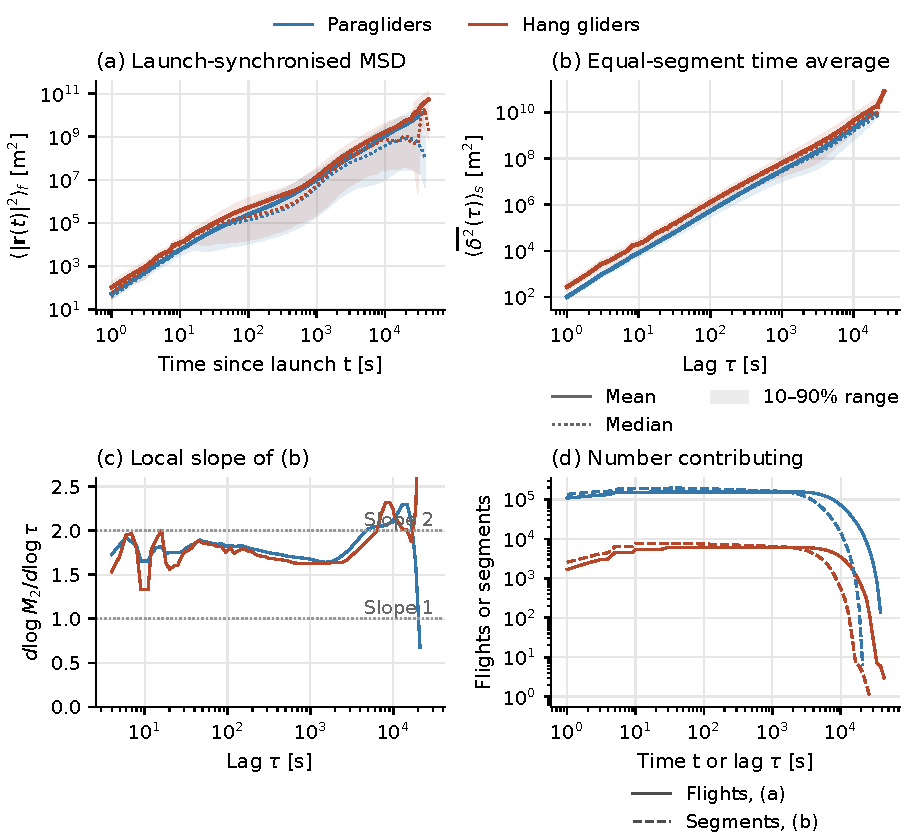
\includegraphics[width=\linewidth]{generated/msd}%
  }{%
    \fbox{\parbox{0.8\linewidth}{\centering\small Figure generated locally by
    \texttt{scripts/reporting/generate\_msd\_figure.py} from the processed dataset on the
    SSD (not versioned). Run \texttt{scripts/preprocess.py} first, then this.}}%
  }
  \caption{\rev{Mean-squared displacement of the retained ensemble
  (\num{\StatMsdParaFlights} paraglider and \num{\StatMsdHangFlights} hang-glider
  flights), by two averages. (a)~The \emph{ensemble} MSD
  $\langle|\mathbf{r}(t)|^2\rangle$ against elapsed flight time, log--log, with the
  fitted straight line dashed, its range shaded, and the \SIrange{10}{90}{\percent} band
  across flights with the median dotted. (b)~The \emph{time-averaged} MSD
  $\overline{\delta^2(\tau)}$, averaged over starting times within each segment and cut
  at half a segment's length. (c)~The local logarithmic slope
  $\mathrm{d}\log\mathrm{MSD}/\mathrm{d}\log t$ of both, over a window of $\pm0.15$
  decades, with the ballistic and diffusive values marked. (d)~The flights, or segments,
  contributing at each lag, on which the upper end of each fit range is set; the rising
  limb is shaded in (a) and (c), where the average is still taken over a growing
  population. Computed by \texttt{scripts/reporting/generate\_msd\_figure.py} from the
  \protect\path{fixes} table; curves written alongside as
  \protect\path{msd_curve.csv}.}}
  \label{fig:msd}
\end{figure}

\section{Segmentation into flight phases}
\label{sec:segmentation}
Building on the previous work of Vilpellet et al.~\cite{vilpellet2026}, each flight is
segmented into the three phases of the soaring cycle:
\begin{description}
  \item[Transition (glide).] The inter-thermal cruise: a near-straight, energy-efficient
        glide toward the next source of lift (sinking, large directed horizontal
        displacement). This is the directed ``step''.
  \item[Search.] The exploratory phase entered when no thermal is found at a comfortable
        altitude: gentle turns and probing manoeuvres to sample the air mass and locate the
        next thermal while limiting altitude loss. It mediates the passage from one step to
        the next trap.
  \item[Climb (thermalling).] Circling within rising air to regain altitude: persistent
        turning with small net horizontal displacement. This is the localized ``trap''.
\end{description}
That work performs the segmentation with a hidden Markov model~\cite{rabiner1989} whose observations are a
small set of \emph{binary} trajectory-derived features --- the sign of the vertical speed,
the persistence of the curvature angle, and indicators of trajectory straightness.

A first task of this thesis is to scrutinize this segmentation rather than take it for
granted: to assess whether those binary variables are adequate and robust on the larger,
more heterogeneous dataset assembled here, and whether the feature set or the model should
be refined, extended, or replaced. The segmentation method is therefore itself an object of
study, and the specific variables are deliberately left open at this stage. This
three-state description refines the two-state caricature underlying continuous-time random
walks and L\'evy walks.

\section{Phase-resolved observables}
\label{sec:phaseobs}
The segmentation gives access to a second group of observables, defined per phase occurrence and
then as ensemble distributions. These are the building blocks of an intermittent-transport
description and, unlike those of Section~\ref{sec:obs-global}, cannot be obtained without
first segmenting the flight.
\begin{description}
  \item[The waiting phase: climb and search.] Between two consecutive glides the flier
        advances little horizontally: it searches for a thermal and climbs in it. For a
        transport model these two phases together form the \emph{waiting time} between
        directed steps, so we treat them on an equal footing and build three distributions --
        the climb duration $\tau_c$, the search duration $\tau_s$, and their sum
        $\tau_w=\tau_s+\tau_c$, the total time spent essentially stationary between glides.
        The distinction matters: Vilpellet et al.~\cite{vilpellet2026} report the
        search times to be broadly \emph{power-law} distributed while the climb times are
        closer to \emph{exponential}, so that the heavy tail of the combined waiting time
        $\psi(\tau_w)$, the quantity that determines whether trapping drives
        sub-diffusion, would be inherited from the search phase. Whether this still holds on
        the larger dataset is itself one of the things to re-check once the segmentation is in
        place. We therefore report $\psi(\tau_w)$ together with the separate $\psi(\tau_c)$ and
        $\psi(\tau_s)$. Alongside the durations we record the climb kinematics (altitude gained
        $\Delta z$, mean climb rate, thermalling radius and period) and the search geometry
        (path length, tortuosity, net displacement) -- the search being the phase in which
        prior work locates the signature of pilot skill.
  \item[The directed step: glide (transition).] Each glide contributes a horizontal step of
        length $\ell$ and duration $\tau_g$, with ground speed, glide ratio (horizontal
        distance per unit altitude lost) and sink rate. Because a glide is close to ballistic,
        $\ell\approx v_g\,\tau_g$, step length and duration are expected to be nearly
        proportional; we test this directly through the joint law of $(\ell,\tau_g)$ -- the
        $\ell$--$\tau_g$ scatter, the conditional mean $\langle\ell\mid\tau_g\rangle$, and the
        spread of the ratio $\ell/\tau_g$ (the glide speed). Both marginals matter: the tail of
        the step-length distribution $\lambda(\ell)$ controls super-diffusive contributions, so
        we compute the distributions of $\ell$ and $\tau_g$ separately as well as their joint
        law.
  \item[Anatomy of a flight.] Number of thermals (climbs) per flight, inter-thermal distances,
        and the fraction of both time and along-track distance spent in each phase: the coarse
        composition that sets the weight of each phase in the global transport.
  \item[Angular diffusion between glides.] The turning angle between the heading of one
        transition segment and the next -- the segment-level counterpart of the turning angle
        of Section~\ref{sec:obs-global}. How fast successive glide directions decorrelate is
        the key ingredient of the minimal model below.
\end{description}

Two couplings then decide which transport model applies, and are stated here as explicit
objects of study. The first is the \emph{step--waiting coupling}: whether a long glide tends
to be followed by a long wait, i.e.\ whether $\ell$ and $\tau_w$ are correlated. A genuine
coupling is the defining feature of a L\'evy walk and is what separates it from a decoupled
CTRW, in which jumps and waiting times are drawn independently.

The second is the \emph{memory in the phase sequence}. A flight is a discrete sequence over
the three states $\{\text{transition},\text{search},\text{climb}\}$, and memory can hide in
two places. (i) The \emph{order} of the phases, summarised by the transition matrix
$P_{ij}=\Pr(\text{next}=j\mid\text{current}=i)$: a perfectly cyclic flight
($\text{T}\!\to\!\text{S}\!\to\!\text{C}\!\to\!\text{T}$) gives a near-deterministic matrix,
whereas aborted climbs, repeated searches or skipped phases appear as off-cycle probabilities
and reveal how stereotyped the soaring cycle actually is. (ii) The \emph{durations}, through
correlations between consecutive phase durations -- for instance whether a long climb tends to
precede a long glide. Both probe the \emph{renewal} assumption underlying the textbook CTRW
and L\'evy-walk results, in which each step and wait is independent of the history: if the
transition matrix is structured or the durations are correlated, the process is non-renewal
and those formulas must be amended. These measurements determine whether a memoryless
model is admissible.

\section{Reproducing the reference results}
\label{sec:reproducing}
A first objective of the analysis, undertaken once the segmentation is in place, is to check
whether the enlarged---and eventually multi-source---dataset reproduces the quantitative and
graphical results of Vilpellet et al.~\cite{vilpellet2026}. That study covers paragliders,
hang gliders and sailplanes; the present data cover the first two (Chapter~\ref{ch:dataset}),
so both the paraglider and the hang-glider comparisons are within reach, while the sailplane
figures become reachable once that source is added. Two figures are the main targets.

The first is the per-phase conditional MSD (their Fig.~3): the transition segments should
stay ballistic ($\alpha=2$, i.e.\ $H=1$) across time lags; the search phase should be
strongly sub-diffusive ($H\approx0.3$ for paragliders and hang gliders, $\approx0.2$ for
sailplanes); and the climb phase should be quasi-ballistic at long lags but with an effective
velocity about two orders of magnitude smaller, including the transient anti-correlation near
the $\sim\!30$\,s thermalling period.

The second is the set of per-phase descriptive statistics (their Fig.~4): the glide ratios
($\approx 8.5$, $10$, and $25$ for paragliders, hang gliders, and sailplanes), the
horizontal-velocity statistics, the heavy-tailed distribution of transition times, the
search-time fraction and the effective search radius, the vertical climb velocities, the
thermalling radii, and the thin, near-exponential distribution of climb times---together with
the global time budget ($\approx\!60\%$ transition, $\approx\!35\%$ climb, the remainder
searching) and the global sub-ballistic scaling ($H\approx0.88$).

Recovering these results would validate the acquisition pipeline and the segmentation and
would test the universality of the reported behaviour on a substantially larger sample;
systematic departures would be equally informative, pointing to dataset- or method-dependent
effects to investigate. This comparison is therefore the bridge between the present
data-acquisition stage and the original analysis that follows.

\section{Modelling and simulation}
\label{sec:modelling}
The aim is a \emph{minimal} stochastic model that reproduces the asymptotic anomalous
scaling reported for soaring (a Hurst exponent $H \approx 0.88$) with as few ingredients as
possible. A preliminary working hypothesis---to be made precise, and possibly revised, once
the empirical phase statistics are available---is that the transport is carried mainly by
the transition (glide) phases. The model would therefore resolve the transition segments
explicitly while merging search and climb into a single effective non-transition state, so
that the soaring cycle reduces to a sequence of directed glides interrupted by
reorientations. Anomalous transport would then emerge from the directed transition segments
combined with an \emph{angular diffusion} of the heading from one transition to the next:
successive glide directions decorrelate gradually rather than abruptly, producing a
correlated random walk whose persistence controls the long-time exponent. Simulated
ensembles would be compared with the data to test whether these ingredients suffice. These
are baseline ideas, to be refined---or changed---as the analysis progresses.

\section{Tooling}
\label{sec:tooling}
Mirror the acquisition package with an analysis package, and let the figures and tables of
this document be generated automatically from the analysis outputs -- as the dataset
statistics already are -- so that this document stays in step with the work and remains a
reliable basis for the thesis and for presentations.
